\documentclass[12pt]{article}
\usepackage[utf8]{inputenc}
\usepackage[english,russian]{babel}
\usepackage[12pt]{extsizes}
\usepackage{booktabs}
\usepackage{graphicx}
\usepackage{graphicx,psfrag}
\usepackage{cite}
\usepackage{sectsty}
\usepackage{amsmath, esint, setspace, fancyhdr, amsfonts, bookmark, blindtext}

\graphicspath{{Figures/}}
\DeclareGraphicsExtensions{.pdf,.png,.jpg}
\setlength{\textheight}{8in}
\setlength{\textwidth}{6.6in}
\setlength{\headheight}{0in}
\setlength{\headsep}{0.2in}
\setlength{\topmargin}{0in}
\setlength{\oddsidemargin}{0in}
\setlength{\evensidemargin}{0in}
\setlength{\parindent}{.3in}
\renewcommand{\baselinestretch}{1.4}

\doublespacing

\begin{document}
\begin{titlepage}

\begin{center}
Санкт-Петербургский политехнический университет Петра Великого\\
Институт прикладной математики и механики\\
Кафедра прикладной математики\\
\hrulefill
\end{center}

\begin{flushleft}
\rule{9cm}{0pt} {Работа допущена к защите}\\
\rule{9cm}{0pt} Зав. кафедрой\\
\rule{9cm}{0pt} \rule{2.5cm}{0.5pt} {\bfseries{М. Е. Фролов }}\\
\rule{9cm}{0pt} "\rule{.9cm}{0.5pt}" \rule{4cm}{0.5pt}
\end{flushleft}

\vspace{1.5cm}

\begin{center}
{\large {\bfseries ОТЧЕТ\\
о научно-исследовательской работе}}\\

\bigskip \bfseries{Тема:} {\bfseries \emph{Классификация саженцев растений}}
\end{center}

\vspace{1.cm}

\begin{flushleft}
Направление: 01.03.02 Прикладная математика и информатика

\vspace{1.cm}

Выполнил студент гр. 33631/4 \hfill{Камалетдинова Ю.А.} \\ 

\vspace{0.2cm} Руководитель \hfill{Яковлев Д.В.}

\end{flushleft}

\vspace{1.5cm}

\begin{center}
Санкт-Петербург\\
2019
\end{center}

\end{titlepage}


\tableofcontents
\addtocontents{toc}{~\hfill\par}
\vfill ~
\setcounter{section}{0}

\section*{Введение}


\section{Анализ набора данных}
\subsection{Первичный взгляд на данные}

\indent{\indentИсследуемый набор данных был собран группой Орхусского университета по обработке сигналов в сотрудничестве в Университетом Южной Дании. В нем содержится приблизительно 960 уникальных изображений растений 12 видов, представленные растения находятся на разных стадиях роста.}\\
\indent{Перед рассмотрением методов классификации изображений целесообрзно проанализировать имеющиеся данные. Так можно существенно улучшить качество результата работы алгоритма.}

\begin{itemize}
	\itemВ ходе изучения набора данных было установлено, что классификацируемые объекты занимают все пространство картинки и дополнительной обрезки не требуется. 
	\itemРаспределение размеров изображений неравномерное, поэтому необходимо привести весь набор к единому разрешению. 
	\itemНезависимо от выбора алгоритма удаление фона изображения позволит существенно улучшить точность определения границы классифицируемого образца
\end{itemize}

\subsection{Предобработка изображений}
\indent{\indentУдаление фона с изображений можен быть реализовано при помощи битового маскирования /* здесь еще дописать */.}\\
\indent{\indentПредставим результат удаления фона на примере выбоки из каждого класса}

\begin{figure}[h]
\centering
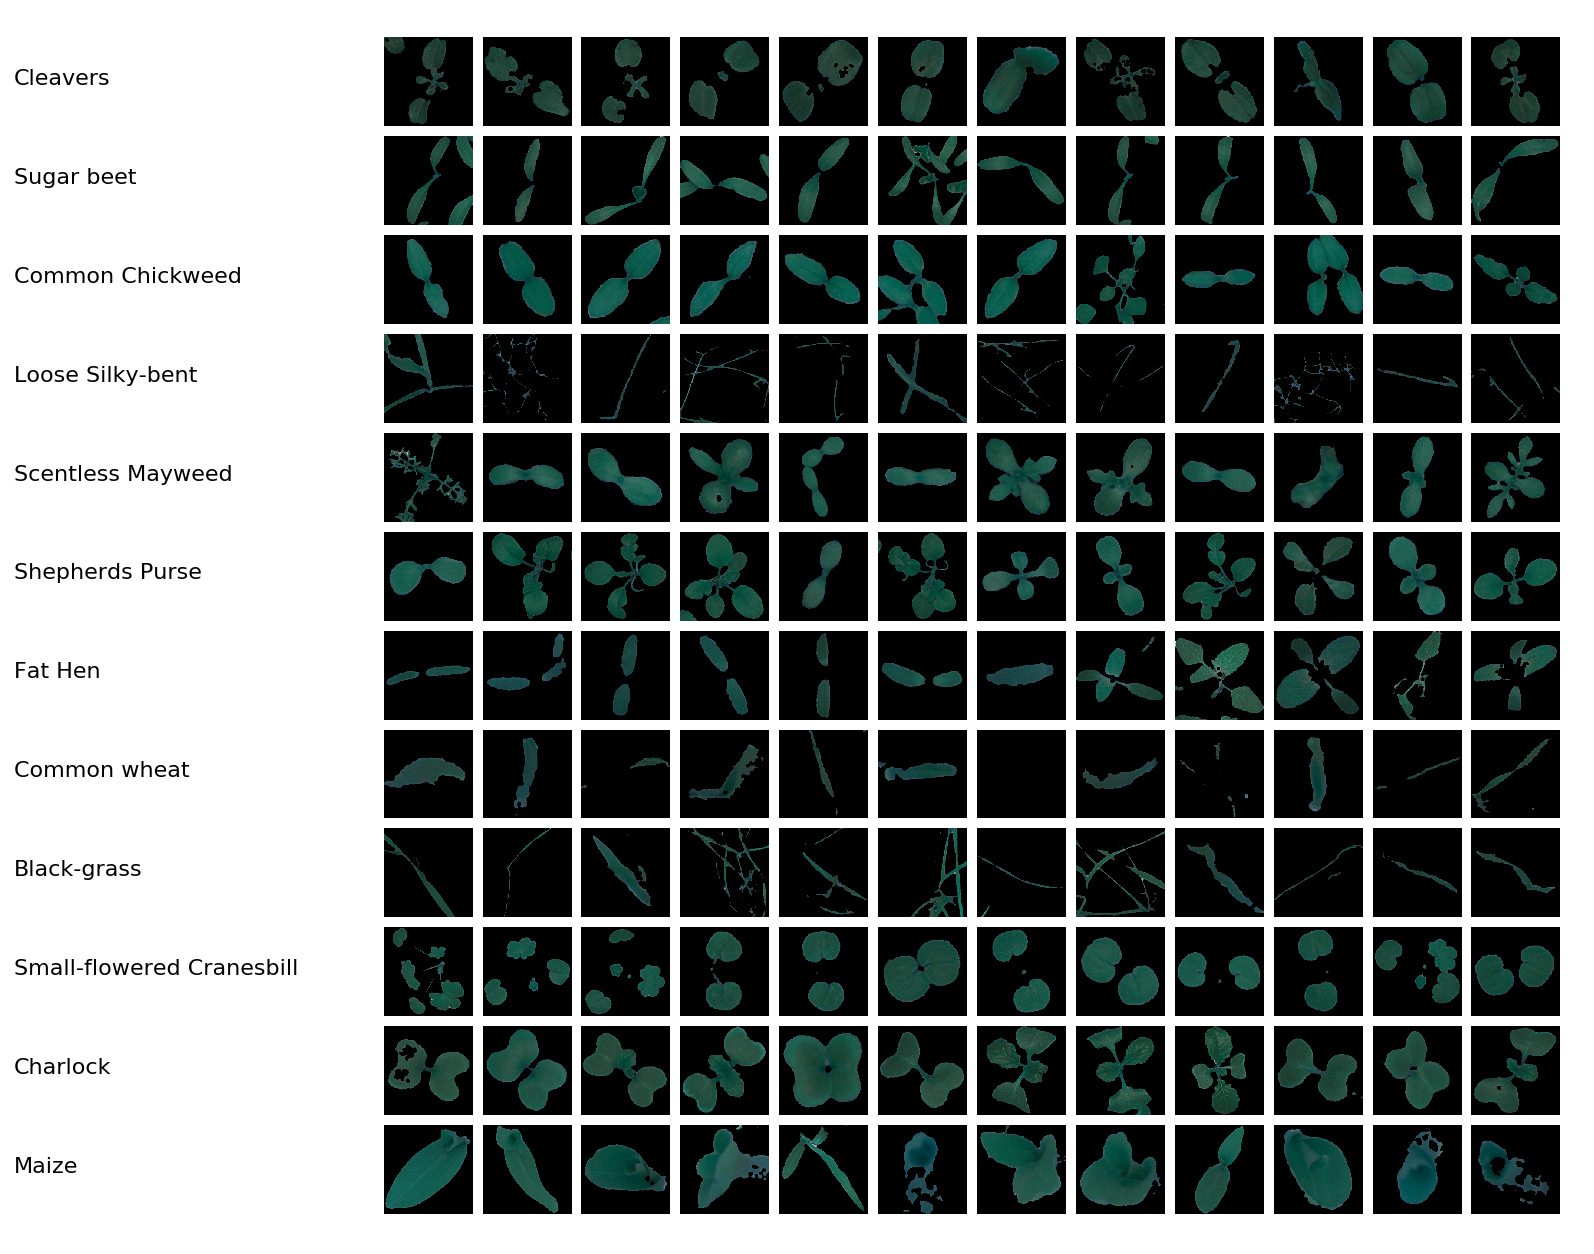
\includegraphics[width=16.cm, height=12.cm]{segmented_part_1}
\end{figure}


\end{document}{}